\documentclass[12pt,a4paper]{article}
% Internationalization 
\usepackage[utf8]{inputenc}
% Better hyphenation for words with digraphs čćžšđ
\usepackage[T1]{fontenc} 
% Set Croatian as active language
\usepackage[croatian]{babel}
% For importing images - .jpg, .png, .pdf, .svg, .eps
\usepackage{graphicx}
% For manualy figure postioning
\usepackage{float} 
% For adding colors to text
\usepackage{color}
% Enabling more defined colors
\usepackage[usenames,dvipsnames]{xcolor}
% Support for .txt listings w/o begin{verbatim}
\usepackage{listings} 
% Pro­vides diffrent formats for \today
\usepackage{datetime}
% For Toc with dots
\usepackage{tocloft} 
% Define geometry
\usepackage[left=2.5cm,top=2.5cm,right=2cm,bottom=2.5cm]{geometry} 
% For fancy headers and footers
\usepackage{fancyhdr} 
% For adding Bibliography in TOC
\usepackage[nottoc]{tocbibind} 
% LaTex has support for simple math formulas 
% For advance mathematical formulas we use
\usepackage{amsmath}
% For setting line spacing e.g. \dobulespacing
\usepackage{setspace}
% Simplifies including multi-page PDF or PS docs
\usepackage{pdfpages}
% For changing title styls with \titleformat
\usepackage[explicit]{titlesec}
% For using hyperlinks 
\usepackage{hyperref}

% Fancy header definition
\pagestyle{fancy}
% Remove default rule in header
\renewcommand{\headrulewidth}{0pt} 
\fancyhf{}
% Set page number in down-right corner of the page
\rfoot{\thepage}

% Change figure name prefix - has to be before \begin{document}
% \addto\captionscroatian{\renewcommand{\figurename}{Sl.}}

\definecolor{myyellow}{HTML}{9100A5}
\definecolor{mygreen}{HTML}{00961B}
\definecolor{myred}{HTML}{B80002}
\definecolor{myblue}{HTML}{1528FF}

% Links style definitions
\hypersetup{
    % fits the width of the page to the window
    pdfstartview={FitH},    
    pdftitle={Prepoznavanje prometnog znakovlja u pokretnoj slici},    
    pdfauthor={Maja Soldo},
    pdfkeywords={OpenCV},
    % false: boxed links; true: colored links
    colorlinks=true,
    pdfborder={0,0,0},
    linkcolor=black,          
    citecolor=mygreen,       
    filecolor=myred,    
    urlcolor=myblue,
}

\begin{document}

% Change section, subsection figure, table. listing numbering
\renewcommand{\thesection}{\arabic{section}.}
\renewcommand{\thesubsection}{\arabic{section}.\arabic{subsection}.}
\renewcommand{\thesubsubsection}{\arabic{section}.\arabic{subsection}.%
\arabic{subsubsection}.}
\renewcommand{\thefigure}{\arabic{section}.\arabic{figure}.} 
\renewcommand{\thetable}{\arabic{section}.\arabic{table}.}
\renewcommand{\thelstlisting}{\arabic{section}.\arabic{lstlisting}.} 

% Change section format style
\titleformat{\section}
  {\Large\bfseries}{\thesection}{1em}{\MakeUppercase{#1}}

% Change listing name
\renewcommand\lstlistingname{Ispis koda} 
\renewcommand\lstlistlistingname{Ispis koda}

\lstset{ %
    backgroundcolor=\color{white},   
    basicstyle=\ttfamily\footnotesize,
    breakatwhitespace=false,         
    breaklines=true,                 
    % captionpos=b,                    
    commentstyle=\color{mygreen},    
    deletekeywords={...},            
    escapeinside={\%*}{*)}, 
    extendedchars=true,              
    frame=single,                    
    keepspaces=true,                 
    keywordstyle=\color{myblue},       
    keywordstyle=[2]\color{myred},
    language=C,
    morekeywords={new},            
    keywords=[2]{imread, VideoCapture, Mat, PCDReader, PCDWriter,
    VoxelGrid, StatisticalOutlierRemoval, search, KdTree, Normal,
    NormalEstimation, PointXYZRGB, PointXYZRGBNormal, PointCloud, Ptr,
    PolygonMesh, Poisson, std, string, io, saveVTKFile, boost, cout,
    concatenateFields, visualization, PCLVisualizer, shared\_ptr,
    posix\_time, microseconds, this\_thread, sleep, PointType,
    PointTypeN},
    numbers=left,                    
    numbersep=5pt,                   
    numberstyle=\textbf\tiny\color{myyellow}, 
    rulecolor=\color{black},         
    showspaces=false,                
    showstringspaces=false,          
    showtabs=false,                  
    stepnumber=2,                    
    stringstyle=\color{myyellow},     
    tabsize=2,                       
    title=\lstname                   
}

\newpage
\begin{titlepage}
\begin{center}

\textbf{\MakeUppercase{\large 
    Sveučilište Josipa Jurja Strossmayera u Osijeku}}\\[0.2cm]

\textbf{\MakeUppercase{\large Elektrotehnički fakultet}}\\[0.8cm]
\textbf{\large Sveučilišni studij}\\ [5cm]

\textbf{\MakeUppercase{\Large 
    Prepoznavanje prometnog znakovlja u pokretnoj slici}}\\ [1cm]

\textbf{\large Završni rad}\\  [5 cm] 

\textbf{\Large Maja Soldo}\\ [0.5cm] 

\vfill

\textbf{\large Osijek, 2014.} \\

\end{center}
\end{titlepage}

% \includepdf[pages={1}]{Obrazac_Z1_04.pdf}
% \includepdf[pages={1}]{izjava_o_originalnosti}
\newpage
% Toc  
\renewcommand{\cftsecleader}{\cftdotfill{\cftdotsep}}
\tableofcontents 
% Set Toc depth - so it doesn't show subsubsections
\addtocontents{toc}{\protect\setcounter{tocdepth}{2}}
% Removing page numbering from this page 
\thispagestyle{empty}

\newpage

\setcounter{page}{1}
\setcounter{figure}{0}
\section{Uvod}% (fold)
\label{sec:Uvod}

\newpage
\subsection{Zadatak diplomskog rada} % (fold)
\label{sub:Zadatak diplomskog rada}

% subsection Zadatak diplomskog rada (end)
% section Uvod (end)

\newpage
\setcounter{figure}{0}

\section{Pregled korištenih tehnologija i algoritama} % (fold)
\label{sec:Tehnologija i teorija}

\subsection{Biblioteka OpenCV} % (fold)
\label{sub:Biblioteka OpenCV}

OpenCV~\cite{opencv_library} (engl. \textit{Open Source Computer Vison})
je biblioteka funkcija odnosno algoritama za matematičku obradu slike i
računalni vid.  Objavljen je pod BSD licencom i stoga je slobodan za
akademske i komercijalne uporabe. Sadrži C++, C, Python i Java sučelja i
podržava Windows, Linux, Mac OS, iOS i Android platforme. OpenCV je
dizajniran za računalnu učinkovitost, sa snažnim naglaskom na stvarno
vremenske aplikacije. Biblioteka je napisana u optimiziranom C/C++ kodu
te može iskoristiti prednosti višejezgrenog procesiranja. Ako se koristi
s OpenCL (engl. \textit{Open Computing Language}) bibliotekom OpenCV
može iskoristi prednosti hardverskog ubrzanja osnovne računalne
platforme.

Usvojen diljem svijeta, OpenCV ima zajednicu korisnika veću od 47 tisuća
ljudi i procijenjeni broj preuzimanja prelazi sedam milijuna. Primjene
variraju od interaktivne umjetnosti, do inspekcija mina, spajanja
internetskih mapa i napredne robotike.

\begin{figure}[h]
\centering

\includegraphics[scale=0.8]{figures/opencv.jpg}
\caption{OpenCV logo}
\label{fig:opencv.svg}
\end{figure}

\newpage
\subsection{Radna okolina} % (fold)
\label{sub:Radna okolina}

U ovom podpoglavlju je dan kratak pregled korištene radne okoline. Pod
radnom okolinom se misli na operacijski sustav, upotrebljavane alate i
programske biblioteke. Tako su izabrane slijedeće komponente:

\begin{description}
  \item[OS:] Ubuntu 12.04
  \item[Biblioteka:] OpenCV 2.4.6
  \item[Prevodioc:] GCC 4.6.3 
  \item[Uređivač teksta:] Geany
\end{description}

Ubuntu 12.04 je izabran zbog stabilnosti, jednostavnog podešavanja i 
dostupnosti velike količine već priprmljenih programskih paketa.
OpenCV 2.4.6 je zadnja stabilna verzija u trenutnku pisanja. Odabrana
je jer se lagano prevodi i instalira na odabranoj verziji Ubuntu OSa.
GCC 4.6.3 je zadna verzija koja dolazi s Ubuntu 12.04 distribucijom.
Geany je uporijebljen zbog svoje jednostavnosti i integracije s GCC
prevoditeljem.
\\


\begin{figure}[!htb]
\minipage{0.32\textwidth}
    
\includegraphics[width=\linewidth]{figures/ubuntu.png}
\endminipage\hfill
\minipage{0.32\textwidth}
    
\includegraphics[width=\linewidth]{figures/gcc.jpeg}
\endminipage\hfill
\minipage{0.32\textwidth}%
    
\includegraphics[width=\linewidth]{figures/geany.jpg}
\endminipage
\caption{Prikaz logotipa upotrebljenih tehnologija}
\end{figure}

% subsection Radna okolina (end)

\newpage
% subsection Biblioteka OpenCV (end)

\subsection{Algoritam usporedbe predloškom} % (fold)
\label{sub:Algoritam usporedbe predloškom}

Postoji više metoda odnosno algoritama koje se koriste za prepoznavanje
različitih objekata na slici. Jedna od njih je algoritam usporedbe s
predloškom (engl. \textit{Template Matching}). U ovom podpoglavlju dan
je primjer korištenja takve metode na mirnoj slici. 

Algoritam usporedbe predloškom je metoda za pronalaženje područja na
slici koji odgovaraju odnosno su slični uspoređenom predlošku. 

Princip rada se zansniva na dvije komponente:
\begin{itemize}
    \item \textbf{Izvorna slika (I)} - slika u kojoj se pronalazi
        odgovarajuća slika predloška.
    \item \textbf{Slika predloška (T)} - manja slika odnosno uzorak koji
        se traži na izvornoj slici.
\end{itemize}

Cilj metode je otkriti najviše odgovarajuća mjesta. Na
slici~\ref{fig:tm1.jpg} vidi se upotreba izvorne slike, slike predloška
i prikaz krajnjeg rezultata metode usporedbe predloškom.

\begin{figure}[h]
\centering
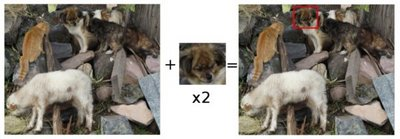
\includegraphics[scale=1]{figures/tm1.jpg}
\caption{Prikaz izvorne slike, slike predloška i krajnjeg rezultata
metode usporedbe predloškom}
\label{fig:tm1.jpg}
\end{figure}

Identificiranje odgovarajućeg područja, radi se uspoređivanjem slike
predloška s izvornom slikom. Pomicanjem predloška piksel po piksel po
izvornoj slici s lijeva na desno, od gore prema dolje kao što je
prikazano na slici~\ref{fig:tm2.jpg}. Na svakoj lokaciji, računa se
vrijednosti koja predstavlja koliko dobro predložak odgovara izvornoj
slici, odnosno koliko su slični.

\begin{figure}[h]
\centering
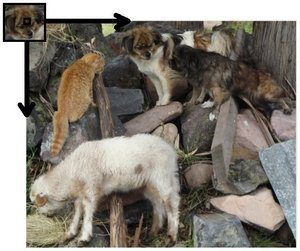
\includegraphics[scale=0.5]{figures/tm2.jpg}
\caption{Prikaz pomicanja predloška po izvornoj slici}
\label{fig:tm2.jpg}
\end{figure}

Za svaku lokaciju piksela u predlošku T preko slike I, pohranjuju se
vrijednosti u matricu rezultata R. Svaka lokacija (x, y) u matrici R
sadrži vrijednosti koja govori koliko je na toj lokaciji predložak
sličan izvornoj slici. 

Slika~\ref{fig:tm3.jpg} prikazuje rezultate R pomicanja predloška po
izvornoj slici. Korištena metoda je \texttt{TM\_CCORR\_NORMED}.
Najsvjetlija mjesta pokazuju odgovarajuće vrijednosti. Kao što se vidi,
mjesto obilježeno crvenim krugom je ono s najvišom vrijednosti. U praksi
se za pronalazk najvećih odnosno najmanjih vrijednosti koristi funkcija
\texttt{minMaxLoc} ovisno o metodi koja se koristi.


\begin{figure}[h]
\centering
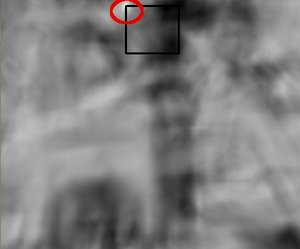
\includegraphics[scale=0.8]{figures/tm3.jpg}
\caption{Prikaz matrice rezultata R nakon usporedbe s predloškom}
\label{fig:tm3.jpg}
\end{figure}

OpenCV funkcija \texttt{matchTemplate} sadržava nekoliko metoda za
računanje rezultantne matrice. Slijede njihove jednadžbe:
\begin{itemize}
    \item \textbf{CV\_TM\_SQDIFF} 
    \item \textbf{CV\_TM\_SQDIFF\_NORMED} 
    \item \textbf{CV\_TM\_CCORR} 
    \item \textbf{CV\_TM\_CCORR\_NORMED} 
    \item \textbf{CV\_TM\_CCOEFF} 
    \item \textbf{CV\_TM\_CCOEFF\_NORMED} 
\end{itemize}

\newpage
\subsubsection{Primjer korištenje funkcije \texttt{matchTemplate} } % (fold)
\label{ssub:Primjer korištenje funkcije }

Slijedi primjer korištenja funkcije \texttt{matchTemplate} za pronalazak
predloška na učitanoj slici.

1. Uključivanje potrebnih zaglavlja i deklaracija varijabli za spremanje
slika i naziv prozora.
\begin{lstlisting}[label=lst1,caption={}]
#include "opencv2/highgui/highgui.hpp"
#include "opencv2/imgproc/imgproc.hpp"
#include <iostream>
#include <stdio.h>
using namespace std;
using namespace cv;
void main () {
Mat img; Mat templ; Mat result;
char* image_window = "Source Image";
char* result_window = "Result window";
int match_method;
\end{lstlisting}

2. Učitavanje izvorne slike i slike predloška preko argumenata predanih
programu.
\begin{lstlisting}[language=,caption={}]
img = imread( argv[1], 1 );
templ = imread( argv[2], 1 );
match_method = argv[3];
\end{lstlisting}

3. Kreiranje prozora za prikaz učitane slike i slike rezultata.
\begin{lstlisting}[language=,caption={}]
namedWindow( image_window, CV_WINDOW_AUTOSIZE );
namedWindow( result_window, CV_WINDOW_AUTOSIZE );
\end{lstlisting}

4. Računanje veličine matrice rezultata i njeno kreiranje.
\begin{lstlisting}[language=,caption={}]
int result_cols =  img.cols - templ.cols + 1;
int result_rows = img.rows - templ.rows + 1;
result.create( result_cols, result_rows, CV_32FC1 )
\end{lstlisting}

5. Pozivanje funkcije matrice rezultata i predvanje potrebnih
argumenata: izvorna slika, slika predloška, matrica rezultata, broj
metode.
\begin{lstlisting}[language=,caption={}]
matchTemplate( img, templ, result, match_method );
\end{lstlisting}

6. Normaliziranje rezultata.
\begin{lstlisting}[language=,caption={}]
normalize( result, result, 0, 1, NORM_MINMAX, -1, Mat() );
\end{lstlisting}

7. Kreiranje varijabli za pronalazak maksimalne i minimalne vrijednost i
lokacije te pozivanje funkcije za pronalazk istih.
\begin{lstlisting}[language=,caption={}]
double minVal; double maxVal; Point minLoc; Point maxLoc;
Point matchLoc;
minMaxLoc( result, &minVal, &maxVal, &minLoc, &maxLoc, Mat() );
\end{lstlisting}

8. Označavanje rezultata pravokutnikom nad 
\begin{lstlisting}[language=,caption={}]
rectangle( img_display, matchLoc, Point( matchLoc.x + templ.cols , matchLoc.y + templ.rows ), Scalar::all(0), 2, 8, 0 );
rectangle( result, matchLoc, Point( matchLoc.x + templ.cols , matchLoc.y + templ.rows ), Scalar::all(0), 2, 8, 0 );
imshow( image_window, img_display );
imshow( result_window, result );

waitKey(0);
}
\end{lstlisting}
% subsubsection Primjer korištenje funkcije tt (end)

% subsection Algoritam usporedbe predloškom (end)

% section Tehnologija i teorija (end)

\newpage
\setcounter{figure}{0}

\section{Prepoznavanje prometnog znakovlja u pokretnoj slici} % (fold)
\label{sec:Prepoznavanje prometnog}

Prepoznavanje prometnog znaka u pokretnoj slici implementirano je u
programu nazvanom \texttt{video-template-matching}. Program se u
potpunosti oslanja na biblioteku OpenCV koja je opisana u
podpoglavlju~\ref{sub:Biblioteka OpenCV} Program se sastoji od pet
logičnih cijelina. 

\begin{itemize}
    \item Učitavanje videa vožnje gradom i učitavanje znaka.
    \item Postavljanje regije interesa na učitanom videu.
    \item Prebacivanje svake sličice iz regije interesa u sličicu sivih
        tonova. 
    \item Obrađivanje takve regije interesa metodom usporedbe s učitanim
        znakom koji je isto slika sivih tonova.
    \item Obrađivanje rezultata, proglašavanje i iscrtavanje pronađenog
        znaka nad svakom sličicom.
\end{itemize}

\begin{figure}[h]
\centering
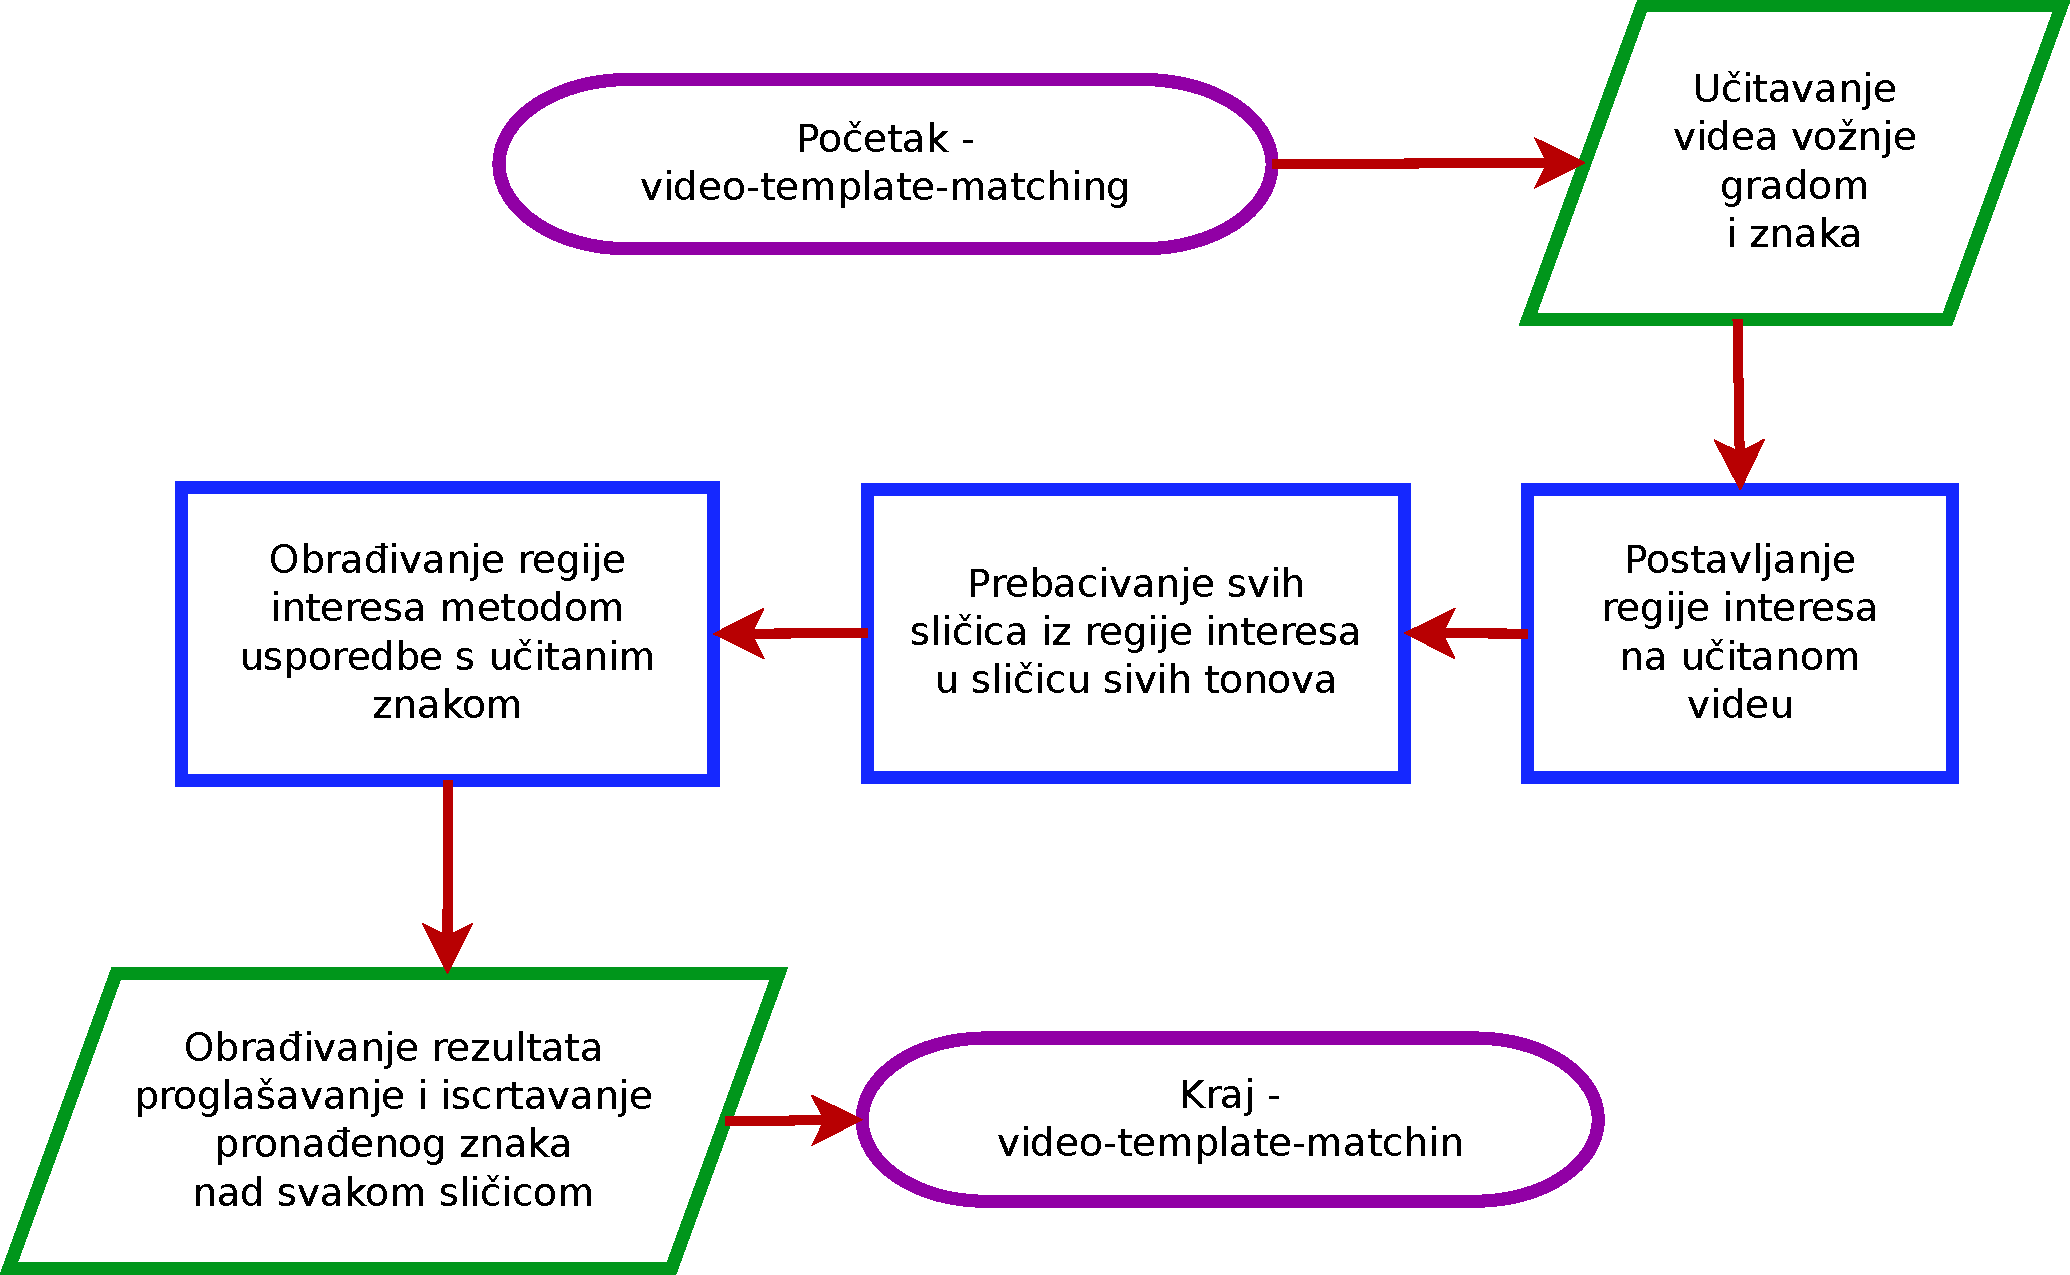
\includegraphics[scale=0.4]{figures/dijagramtoka.pdf}
\caption{Dijagram toka programa video-template-matching}
\label{fig:dijagramtoka.pdf}
\end{figure}


\newpage
\subsection{Učitavanje videa vožnje i učitavanje znaka} % (fold)
\label{ssub:Učitavanje videa vožnje i učitavanje znaka}

\begin{lstlisting}[label=lstUcit,caption={Izvorni kod za učitavanje
videa i znaka}]
#include "opencv2/imgproc/imgproc.hpp"

int main (int argc, char *argv[])
{
    // kreiranje objekta cap za ucitavanje videa
    VideoCapture cap("video/znakich2.mp4");
    if(!cap.isOpened())  // provjera uspjeha ucitavanja
        return -1;

    // kreiranje objekta Mat za spremanje znakova
    Mat znak1, znak2, znak3, znak4;

    // ucitavanje izrezanih znakova u razlicitim velicinama
    // trenutno se koristim samo znak2 
    znak1 = imread ("roi/01_roi.png");		
    znak2 = imread ("roi/02_roi.png");
    znak3 = imread ("roi/03_roi.png");
    znak4 = imread ("roi/04_roi.png");

    return 0;
}
\end{lstlisting}

Izlistanje koda~\ref{lstUcit} prikazuje primjer učitavanja videa i
učitavanje znaka upotrebom klase \texttt{VideoCapture} i funkcije
\texttt{imread} koji su uključeni dodavanjem biblioteke
\texttt{imgproc.hpp}. Kreiranom objektu \texttt{cap} predana je putanja
do videa kojeg treba učitati. Ukoliko video nije uspješno učitan program
završava i vraća \texttt{-1}. Kreiranim objektima \texttt{znak1},
\texttt{znak2}, \texttt{znak3}, \texttt{znak4} pridjeljene su slike
učitane upotrebom funkcije \texttt{imread} kojoj je predana putanja do
slike koju treba učitati.



% subsection Učitavanje videa vožnje i učitavanje znaka (end)


% section Prepoznavanje prometnog (end)

\newpage
\setcounter{figure}{0}

\section{Rezultati} % (fold)
\label{sec:Rezultati}

U ovom poglavlju prikazani su rezultati rada razvijenog programa za
prepozavanje statičnog znaka iz snimke prometnice vozila u pokretu.  Za
ispitivanje funkcionalnosti metode odabrana je jedna scena voženje i
jedan znak kojeg metoda treba pronaći. Znak je prikazan na
slici~\ref{fig:znak}, a scena vožnje je snimljena na osječkoj
obilaznici i prikazana na slici~\ref{fig:scena.png}.

\begin{figure}[h]
\centering

\includegraphics[scale=0.5]{figures/znak.png}
\caption{Prikaz korištenog znaka - obvezan smjer kretanja u desno}
\label{fig:znak}
\end{figure}

\begin{figure}[h]
\centering
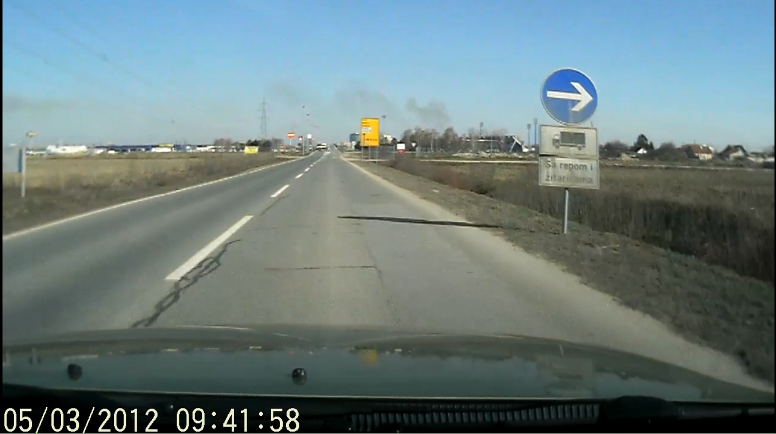
\includegraphics[scale=0.3]{figures/scena.png}
\caption{Prikaz testirane scene voznje}
\label{fig:scena.png}
\end{figure}

\newpage
\subsection{Prikaz rezultata} % (fold)
\label{sub:Prikaz rezultata}

Rezultati su prikazani na slikama s dva prozora. U prvom prozoru
prikazana je regija interesa sa scene unutar koje algoritmom usporedbe
tražimo znak. Regija interese je odabrana na temelju pretpostavke da će
pozcija znaka bit s desne strane učitane scene. Također regija interesa
se definira kako bih se smanjila količina podataka koju algoritam mora
obraditi. U drugom prozornu prikazana je matrica rezultata koju metoda
koristi za pronalazak znaka.  Postoji nekoliko tipova rezultata:
pozitivni, negativni i lažno pozitivni. Svi tipovi rezultata su
predstavljeni dalje u tekstu. Slika~\ref{fig:01} prikazuje sličicu iz
videa sa scene na kojoj nema znaka niti ga je metoda/program našao što
je pozitivan rezultat.

\begin{figure}[h]
\centering
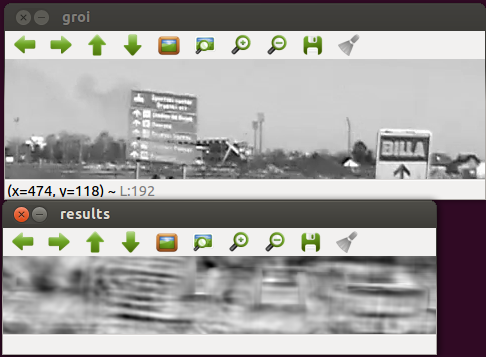
\includegraphics[scale=0.5]{figures/01.png}
\caption{Prikaz sličice videa i rezultata - pozitivan rezultat}
\label{fig:01}
\end{figure}

Lažno pozitivni rezultat prikazuje slika~\ref{fig:02} na kojoj je metoda
pronašala znak gdje nije trebala. Takvi rezultati su očekivani ali nisu
poželjni te ih se pokušalo smanjiti na što manji broj metodom opisanom 
u podpoglavlju~\ref{ssub:Eliminacija lažno pozitivnih rezultata}

\begin{figure}[h]
\centering
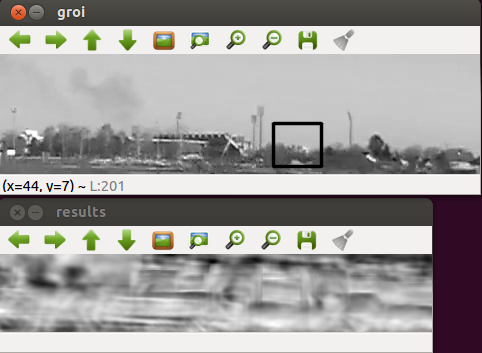
\includegraphics[scale=0.5]{figures/02.png}
\caption{Prikaz sličice videa i matrice rezultata - lažno pozitivan
rezultat}
\label{fig:02}
\end{figure}

\newpage
\begin{figure}[h]
\centering
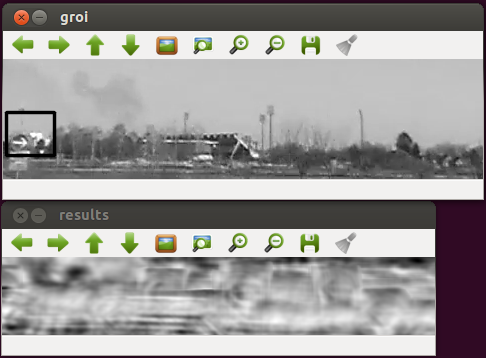
\includegraphics[scale=0.5]{figures/03.png}
\caption{Prikaz sličice videa i matrice rezultata - pozitivan rezultat }
\label{fig:03.png}
\end{figure}

Na slikama~\ref{fig:03.png}, \ref{fig:04.png} i \ref{fig:05.png} vidi se
da je metoda uspješno pronašla znak na različitim udaljenostima odnosno
veličinama znaka iako se koristila samo jedna veličina znaka za
pronalazak. Metoda odnosno program bih se mogao unaprijediti tako da se
ugradi uspoređivanje s različitiim veličinama predloška odnosno znaka.

\begin{figure}[!htb]
\minipage{0.5\textwidth}
    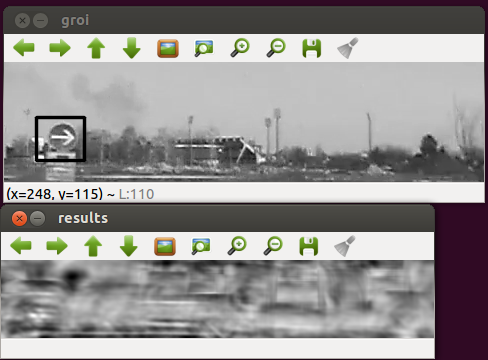
\includegraphics[width=\linewidth]{figures/04.png}
\endminipage\hfill
\minipage{0.5\textwidth}
    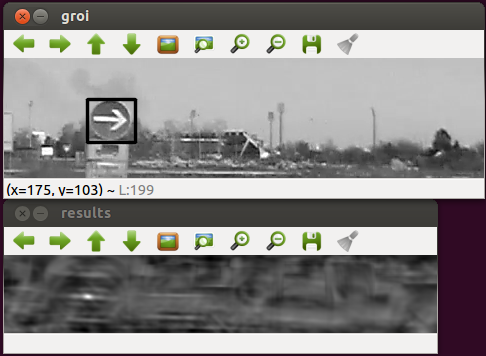
\includegraphics[width=\linewidth]{figures/05.png}
\endminipage\hfill
\caption{Prikaz sličice videa i matrice rezultata - pozitivan rezultat}
\label{fig:04.png}
\end{figure}

Matematička metoda korištena u algoritmu prikazuje pozitivne rezultate
bijelom bojom te se na slici~\ref{fig:04.png} jasno mogu vidjeti
"žarišta" u matrici rezultata.

\newpage

Slika~\ref{fig:06.png} također prikazuje uspješan pronalazak znaka kada
je i znak na izvornoj slici nešto veći nego na slici predloška.
Slika~\ref{fig:07.png} prikazuje negativan rezultat iako se na slici s
rezultatima može vidjeti "žarište" na lokaciji gdje je znak. Program se
može unaprijediti da prati relativne vrijednosti u matrici rezultata i
na taj način bi se takvi negativni rezultati mogli smanjiti.

\begin{figure}[h]
\centering
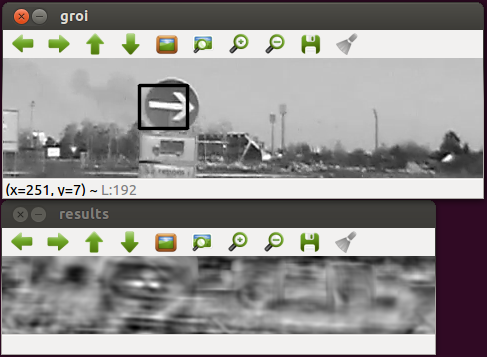
\includegraphics[scale=0.5]{figures/06.png}
\caption{Prikaz sličice videa i matrice rezultata - pozitivan rezultat}
\label{fig:06.png}
\end{figure}

\begin{figure}[h]
\centering
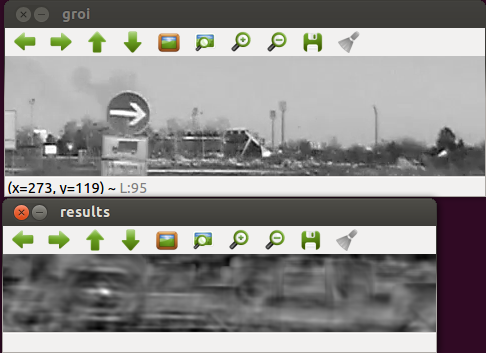
\includegraphics[scale=0.5]{figures/07.png}
\caption{Prikaz sličice videa i matrice rezultata - negativan rezultat}
\label{fig:07.png}
\end{figure}


% subsection Prikaz rezultata (end)
% section Rezultati (end)

\newpage
\setcounter{figure}{0}

\section{Zaključak} % (fold)
\label{sec:Zaključak}

% section Zaključak (end)

%\newpage
% Removing page numbering from this page but not from showing up on TOC
\thispagestyle{empty}

\bibliography{12-bibliography}{}
\bibliographystyle{plain}

\newpage
\thispagestyle{empty}

\section*{Sažetak} % (fold)
\addcontentsline{toc}{section}{Sažetak}
\label{sec:Sažetak}

U ovom radu implementirana je i prikazana jedna od metodologija
računalnog vida za pronalazak prometnog znaka u pokretnoj slici.
Napisani program upotrebljava algoritam usporedbe s predloškom za
pronalazak znaka u zadanoj pokretnoj slici. Program se oslanja na mnoge
funkcije iz OpenCV biblioteke za pronalazak znaka. Rezultati rada
programa su predstavljeni, opisane su prednosti i nedostatci odabrane
metode te su dani prijedlozi za daljnja unaprijeđenja.
\\[0.5cm]

\noindent\textbf{Ključne riječi:} OpenCV, procesiranje videa, usporedba
s predloškom, obrada slike.

\section*{Abstract} % (fold)
\label{sec:Abstract}

The aim of this study was to implement one of computer vision
methodologies for finding traffic sign in motion picture. Developed
program uses template matching algorithm for finding sign in given
motion picture. Program is based on many OpenCV library functions. 
Results of developed program are presented, advantages and
disadvantages of used method are described and also propsitions for
further improvements are given.
\\[0.5cm]

\noindent\textbf{Keywords:} OpenCV, Video processing, template matching,
image processing.

% section Sažetak (end)

\newpage
\thispagestyle{empty}

\section*{Životopis} % (fold)
\addcontentsline{toc}{section}{Životopis}
\label{sec:Životopis}

Maja Soldo rođena je 22. kolovoza 1988. godine u Beogradu. Godine 1995.
upisuje osnovnu školu Antuna Mihanovića u Osijeku. Nakon završetka
osnovne škole upisuje I. gimnaziju u Osijeku. Godine 2007. polaže maturu
s vrlo dobrim uspjehom i upisuje Preddiplomski studij računarstva na
Elektrotehničkom fakultetu u Osijeku. Tijekom studija je radila u
Hrvatskom Telekomu, Ypsilon produkciji, a sada radi kao instruktor
funkcionalnog treninga.
\\[1cm]

\hfill{\textbf{Potpis:}}
% section Životopis (end)

\newpage

\section*{Prilozi} % (fold)
\addcontentsline{toc}{section}{Prilozi}
\label{sec:Prilozi}

\subsubsection*{Izlistanje koda} % (fold)
\label{ssub:Izlistanje koda}

% subsubsection Izlistanje koda (end)

% section Prilozi (end)


\end{document}
